\documentclass[a4paper,english,12pt,bibliography=totoc]{scrreprt}
\setlength{\parindent}{0pt}
\usepackage[T1]{fontenc} %immer
\usepackage[utf8]{inputenc} %am
\usepackage{babel} %Anfang

\usepackage{enumitem} %Aufzählungen verändern

%Gleichungen verwenden
\usepackage{newtxtext}
\usepackage{amsmath}
\usepackage{amssymb}
\usepackage{mathptmx}
%\usepackage{txfonts}

\usepackage{listings}% code blocks
\usepackage[most]{tcolorbox}

%Querverweise
\usepackage{varioref} %immer
\usepackage{hyperref} %in dieser
\usepackage{cleveref} %Reihenfolge

\usepackage{booktabs} %schönere Tabellen
\usepackage{siunitx} %SI-Einheiten
\usepackage{tabularx} %Tabellen mit flexiblen Spalten	

\usepackage{graphicx} %Grafiken verwenden

\usepackage{lipsum} %Blindtext
\usepackage{subcaption}
\usepackage{afterpage}
\usepackage[headsepline]{scrlayer-scrpage} %Paket für Kopfzeilen
\usepackage{afterpage}
\usepackage{float}
\automark[subsection]{section}

\pagestyle{scrheadings}
\ihead{} % oben links
\chead{\leftmark} % oben Mitte
\ohead{} % oben rechts
\cfoot{\pagemark} % unten Mitte
\automark[section]{section} % Modified line

% Zu volle hboxen korrigieren
\tolerance 1414
\hbadness 1414
\emergencystretch 1.5em
\hfuzz 0.3pt
\widowpenalty=10000
\vfuzz \hfuzz
\raggedbottom

%Informationen über das Dokument
\date{\today}


\begin{document}


\begin{titlepage}
	\centering
	
\includegraphics[width=0.8\textwidth]{logo_uulm_sw}
	
	\vspace{1cm}
	\LARGE Compulsory Module for Master Programs
	\Huge \textbf{Biophysics Lab Course}
	
	\vspace{1cm}
	\Large Experiment:

	\Huge \textbf{Protein crystalization}
	
	\vspace{15mm}
	\Large Performed on 11.12.2023
	
	\vspace{5mm}
	\LARGE Group 8
	
	\vspace{1cm}
	\Large
	\begin{tabular}{rcl}
	\textbf{Haiyang Zhang} & and & \textbf{Nicolae Turcan}\\
	\href{mailto:student.1@uni-ulm.de}{haiyang.zhang@uni-ulm.de} & & \href{mailto:student.2@uni-ulm.de}{nicolae.turcan@uni-ulm.de}
	\end{tabular}
	
	\vspace{7mm}
	Supervisor: David Sinn
	
	\vfill
	\begin{tabular}{p{50mm}@{\hspace{5cm}}p{50mm}}
	%\centering \underline{Haiyang Zhang} & \centering \underline{Nicolae Turcan} 
	%\hrulefill & \hrulefill 
	\end{tabular}
	
	\vspace{5mm}
	\normalsize \raggedright
	We hereby confirm that we have elaborated the present work independently and have detailed knowledge of the entire contents.
\end{titlepage}

\tableofcontents

\chapter{Introduction}

 In the 19th century, protein crystallization was developed as a powerful purification tool and demonstration of chemical purity. Single protein crystals are necessary for X-ray and neutron diffractions, which are essential techniques to yield atomic level structures of biological macromolecules\hyperref[sec:ref_1]{[1]}. However, unlike the procedure of acquiring some simple inorganic crystals, protein crystallization has two challenges.\\


\begin{figure}[H]
        \centering
        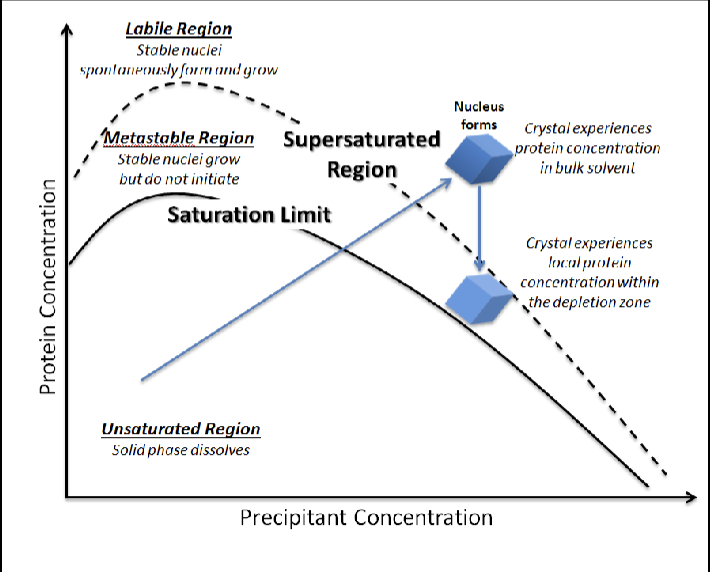
\includegraphics[width=0.9\textwidth]{2. First draft of protein crystalization/Images/Crystalization curves.png}
	    \caption{Phase diagram for the description of protein crystallization\hyperref[sec:ref_2]{[2]}}
\end{figure}

First, very pure protein solution is a necessary prerequisite for the crystallization. However, the purification of protein is difficult. Compared to the elements of ordinary inorganic crystals, proteins exhibit more complex structures, making the formation of periodic structures more challenging. Proteins are highly susceptible to temperature and acidity, and they are easy to degradation. Consequently, purifying proteins without compromising their structural integrity and biological activity becomes a challenging task. In this case, many purification strategies are made on the basis of the unique physical and chemical properties, and the 3-D structures of the target proteins.\hyperref[sec:ref_3]{[3]}.\\

Furthermore, overcome the nucleation barrier is another challenge in protein crystallization. Generally speaking, supersaturated solutions are necessary for the nucleation. However, it is more likely to form many small crystals instead of large crystals if the solution is supersaturated throughout the entire process. In order to grow large crystals, the solution should be kept in the metastable region, where no nuclei will be formed. As is shown in the figure 1.1\hyperref[sec:ref_4]{[4]}, the approach involves initiating nucleation in a supersaturated state initially. Subsequently, the solution is carefully manipulated to transition into a metastable state, fostering the growth of crystals.\\

In our experiment, we used the vapor diffusion techniques(see methods part) to control the solution of the protein, and by attempting different combinations of NaCl solution( 4\%, 5\%, 6\%, 7\%, 8\%, 9\% in the buffer) and sodium acetate(250mM, pH 4.0, 4.4, 4.8, 5.2), which alter the solubility of the protein.  We aimed to identify the optimal conditions regarding these factors for protein crystallization.

\chapter{Materials and methods}

\section{Materials}

\begin{table}[h]
\centering
\begin{tabular}{|c|c|}
  \hline
  Material name & model \\
  \hline
  Lysozyme in \(\mathrm{H_2O }\) & 20 mg/ml \\
    \hline
  NaCl solution & 20\%  \\
    \hline
  Distilled water &  \\
    \hline
Sodium acetate & 250mM, pH4.0\\
  \hline
  Sodium acetate & 250mM, pH4.4\\
  \hline
  Sodium acetate & 250mM, pH4.8\\
  \hline
  Sodium acetate & 250mM, pH5.2\\
  \hline
  FutureWinJoe & \\
  \hline
\end{tabular}
\caption{Materials}
\label{tab:material}
\end{table}

\begin{figure}[H]
        \centering
        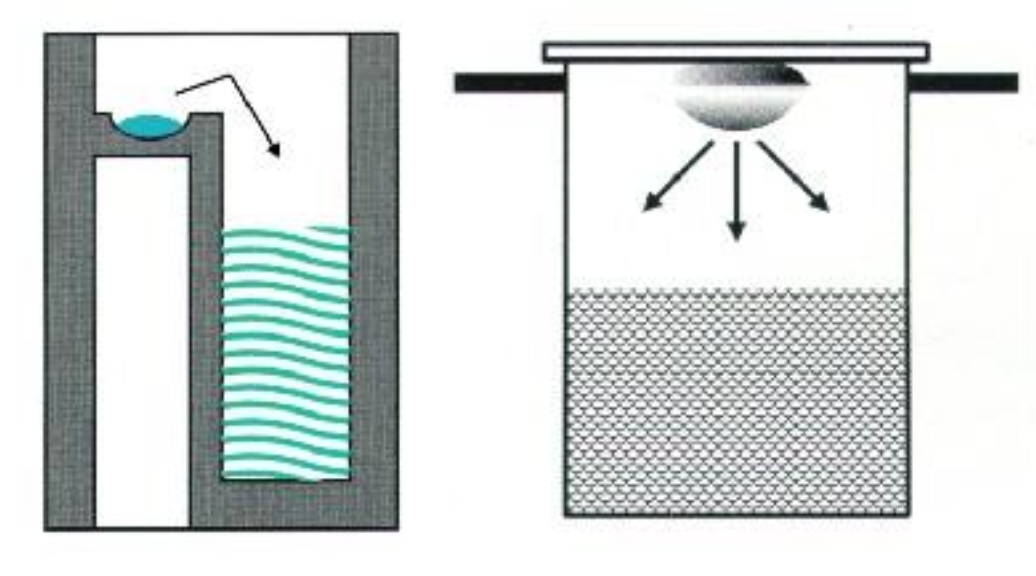
\includegraphics[width=0.8\textwidth]{2. First draft of protein crystalization/Images/Vapour diffusion techniques.png}
	    \caption{The vapor diffusion crystallization techniques: sitting drop(left) and hanging drop(right)\hyperref[sec:ref_2]{[2]}}
\end{figure}

\begin{figure}[H]
        \centering
        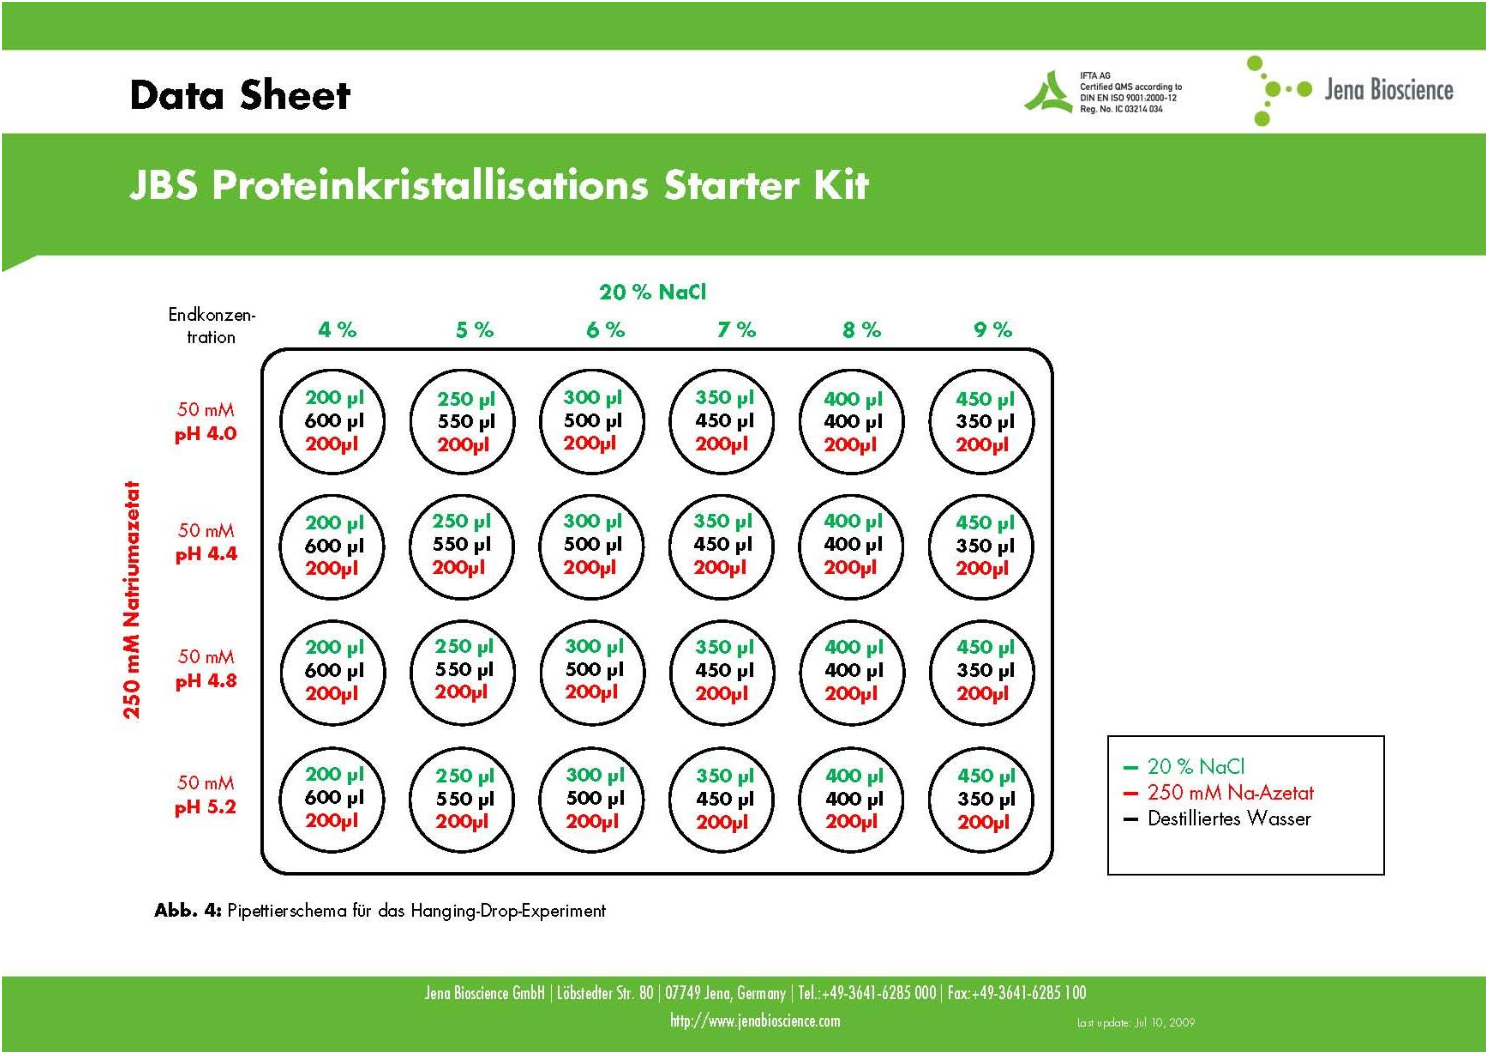
\includegraphics[width=0.8\textwidth]{wells}
	    \caption{pH and NaCl concentration of buffer in each well\hyperref[sec:ref_3]{[3]}}
\end{figure}

\section{Methods}
In this experiment, a vapor diffusion technique was used\hyperref[sec:ref_4]{[4]}.(Figure 2.1) In this technique, a droplet mixed with purified protein, buffer and precipitant is sealed together in a chamber. The transfer of water from the droplet to reservoir will happen because of the 
droplet have a higher concentration of precipitant. As the concentration of protein in the droplet increasing, the nucleation barrier is exceeded, which is necessary for nucleation. After that, the concentration of protein solution will decrease, and ideally it will approach the metastable region, and starting to form the large crystal. In the figure 2.1, two methods(sitting drop and hanging drop) are shown in the figure, and hanging drop method is applied in our experiment.\\


In this experiment, we pipette three different solutions into the \(4 \times 6\)  well plate according to the figure 2.2, then we put a ring of silicone grease around each well. After that, 1\(\mu l\) of protein solution and 1\(\mu l\) of buffer from the respective well are mixed on the middle of the cover slip. More over, we turn over the cover slips and place them on each well. Finally, we put the plate under room temperature for protein crystallisation.\\


After 48 hours, we visually examine the droplet to identify large crystals. Following this, we inspect the droplet using an optical microscope to capture  crystal images under higher resolution. With the assistance of FutureWinJoe, we can view these images on a monitor and record them for further analysis.\\


\chapter{Result and discussion}
After 48 hours, we could not find any protein crystal by direct inspection. However, we observed some differences about the size of crystals and the distribution of the protein crystals in the solution using FutureWinJoe. The results are demonstrated in the table 3.1.

\begin{table}[h]
\centering
\begin{tabular}{|c|c|c|c|c|c|c|}
  \hline
   concentration of NaCl/ pH& \%4 & \%5 & \%6 & \%7 &\%8 & \%9 \\
    \hline
	pH 4.0 &Ms &Ms & Ms& Ms+Fl &Ms+Fl &Ss+Fl \\
  \hline
  	pH 4.4 &Ss+Fl &Ms &Ms+Fl &Ms &Ms &Ss+Fl \\
  \hline
        pH 4.8 &Ms+Fl &Ms &Ms & Ms+Fl&Ms+Fl & Ms+Fl\\
  \hline
        pH 5.2 &Fs+Fl &Fs & Ms &Ms &Ms &Fs \\
  \hline
\end{tabular}
\caption{Numbers and size of protein crystals in each well, M means many, S means some, F means few, l means large, s means small. For example, Ms+fl means in the drop there are many small crystals and a few of large crystals in this droplet.}
\end{table}


In this context, 'many' indicates that the droplet is nearly fully occupied by crystals, while 'some crystals' suggests a more dispersed distribution. 'Few' signifies that only a small number of crystals are present within the droplet. In terms of crystal size, 'small' refers to crystals with a size smaller than 50 $\mu$m, whereas 'large' indicates crystals larger than 50$\mu$m. Examples illustrating these distinctions are presented in Figure 3.1.


\begin{figure}[H]

    \begin{subfigure}{0.45\textwidth}
        \centering
        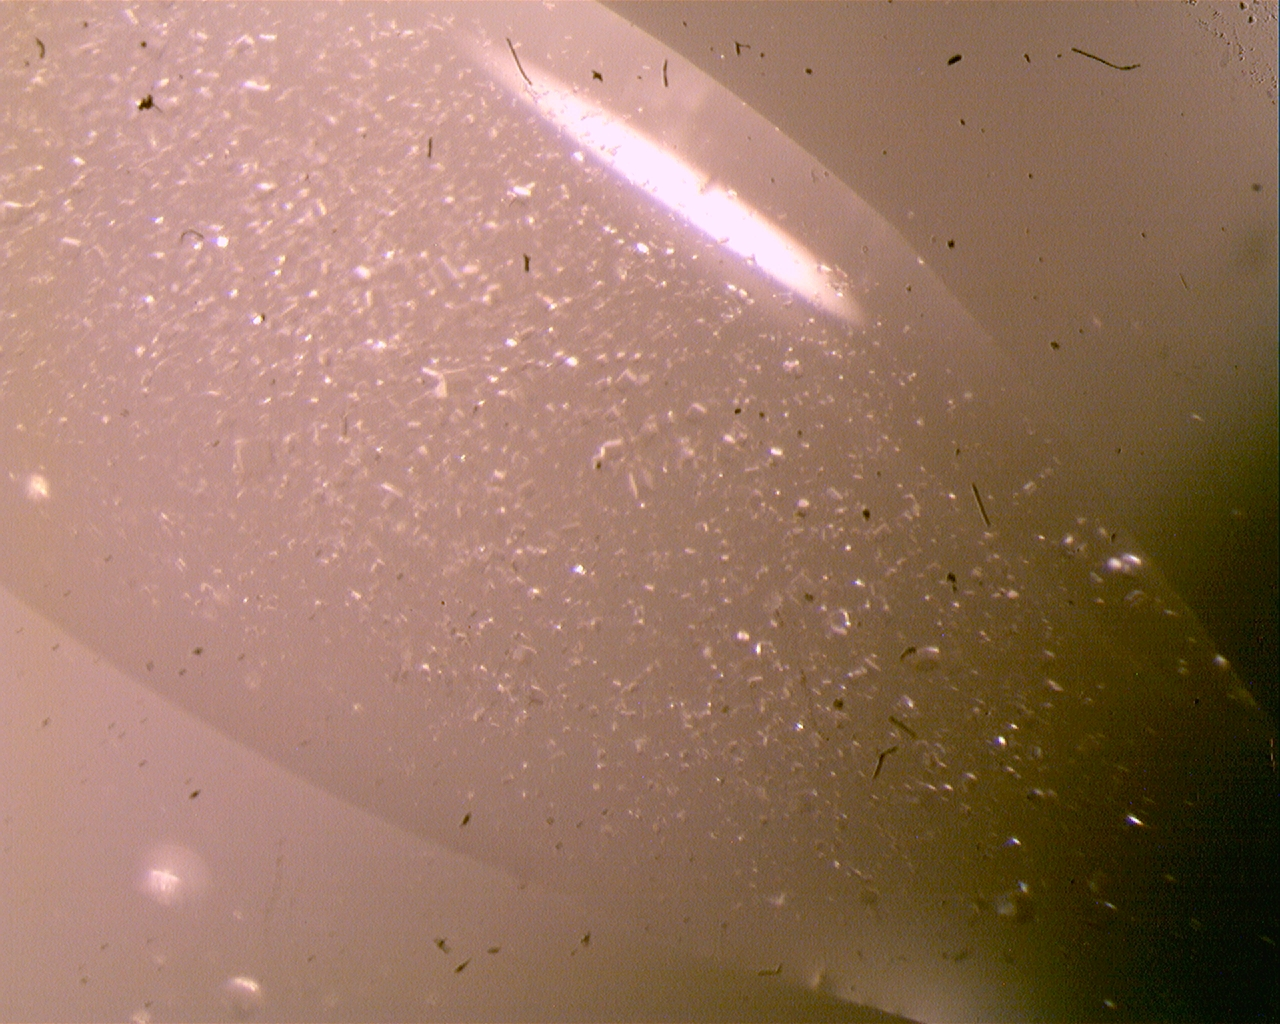
\includegraphics[width=\textwidth]{2. First draft of protein crystalization/Images/Image-6_2000-01-21.jpg}
        \caption{The crystal distribution in the droplet where pH = 4.4 and concentration of NaCl = 4\%}
        \label{fig:pH4.4,4ptg}
    \end{subfigure}
    \begin{subfigure}{0.45\textwidth}
        \centering
        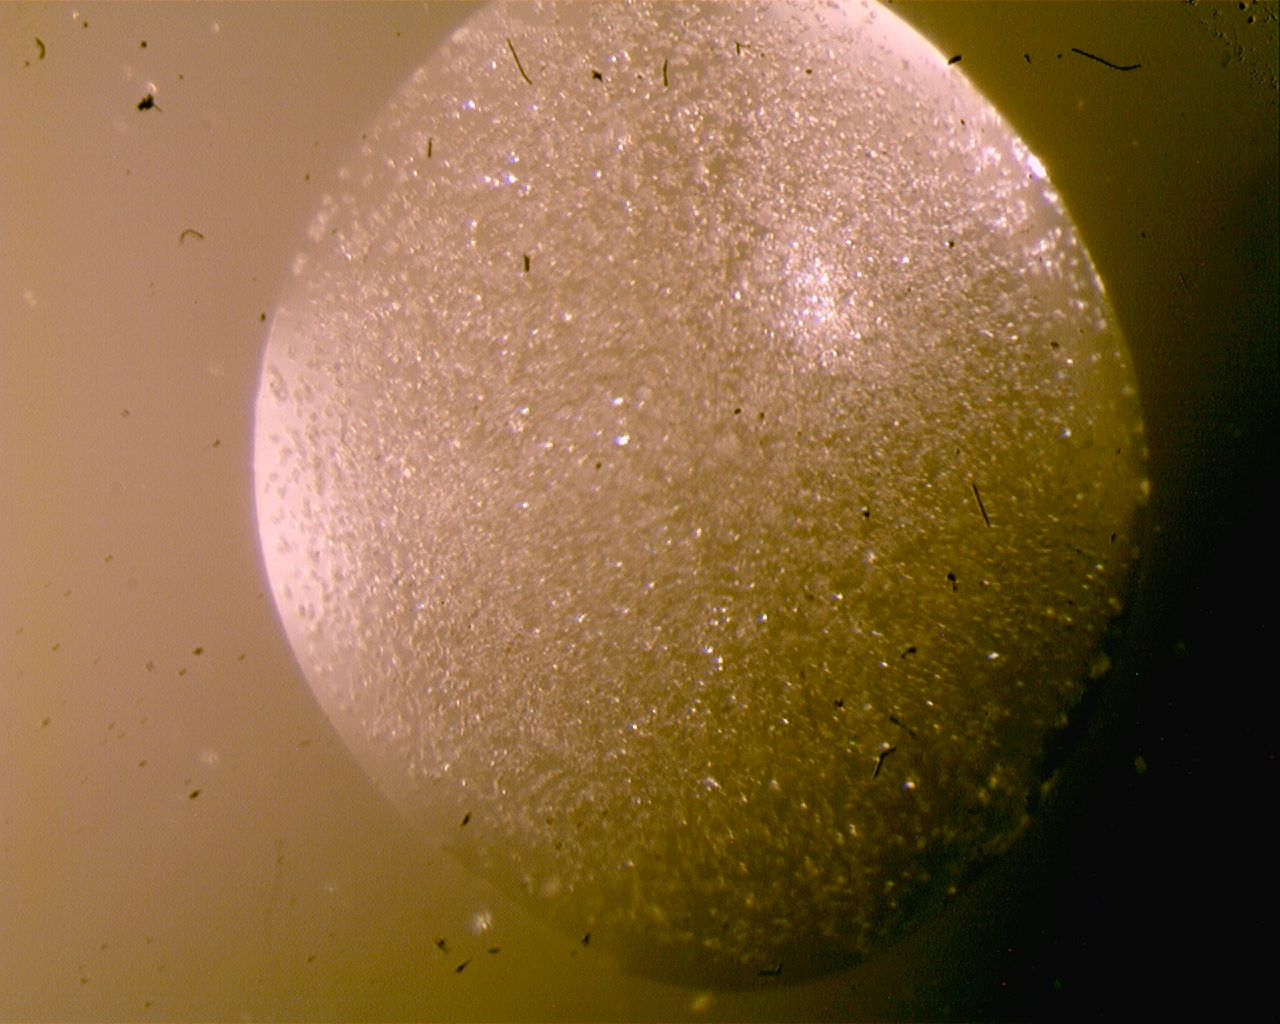
\includegraphics[width=\textwidth]{2. First draft of protein crystalization/Images/Image-9_2000-01-21.jpg}
        \caption{The crystal distribution in the droplet where pH = 4.4 and concentration of NaCl = 7\%}
        \label{fig:pH4.4,7ptg}
    \end{subfigure}
    \caption{The crystal distribution in the droplet. The left one is described as some small crystals and few large crystals; the right one is described as many small crystals. }
    \label{fig:ym_cp_curve}
    
\end{figure}

According to previous research, the pH and the concentration of NaCl solution has evident influence on the solubility of protein\hyperref[sec:ref_5]{[5]}. Applying the mechanics of crystallization mentioned in the introduction part, we are giving a brief discussion on the results shown in table 3.1.\\

After the transfer of water molecules into the chamber, nucleation occurs in the supersaturated region. In this process, crystal nuclei form. Subsequently, as the protein concentration decreases, the protein solution reaches the metastable region. Here, the crystals begin to grow larger, and growth halts when the concentration of the solution equals the saturation limit. The description and analysis of each group (separated by pH) is as follows:\\


-pH = 4.0: In terms of the number of crystals in the images, many small crystals were observed under the concentration of NaCl from 4\% to 8\%. However, there was a decrease in the number of crystals(some crystals) at 9\% NaCl. As for crystal size, from the 7\% NaCl to 9\% NaCl, a few large crystals appeared. According to the phase diagram, the presence of crystals indicates that the protein solution entered the supersaturated region. The emerging of large crystals from 7\% to 9\% NaCl suggests that these protein solutions reached the metastable region after some crystals precipitated, potentially signalling an increase in protein solubility.


%The previous study\hyperref[sec:ref_5]{[5]} shows that the solubility of protein has a positive correlation 
%-pH = 4.0: All protein solutions start in the supersaturated region. Between 4\% NaCl and 6\% NaCl, the solubility of the protein is relatively low as the solution remains in the supersaturated region post-nucleation. However, from the 7\% NaCl, as the concentration of the NaCl solution increases, the solubility of the protein also increases. The protein solution transitions into the metastable region, leading to the formation of large crystals.\\

\begin{figure}[H]
        \centering
        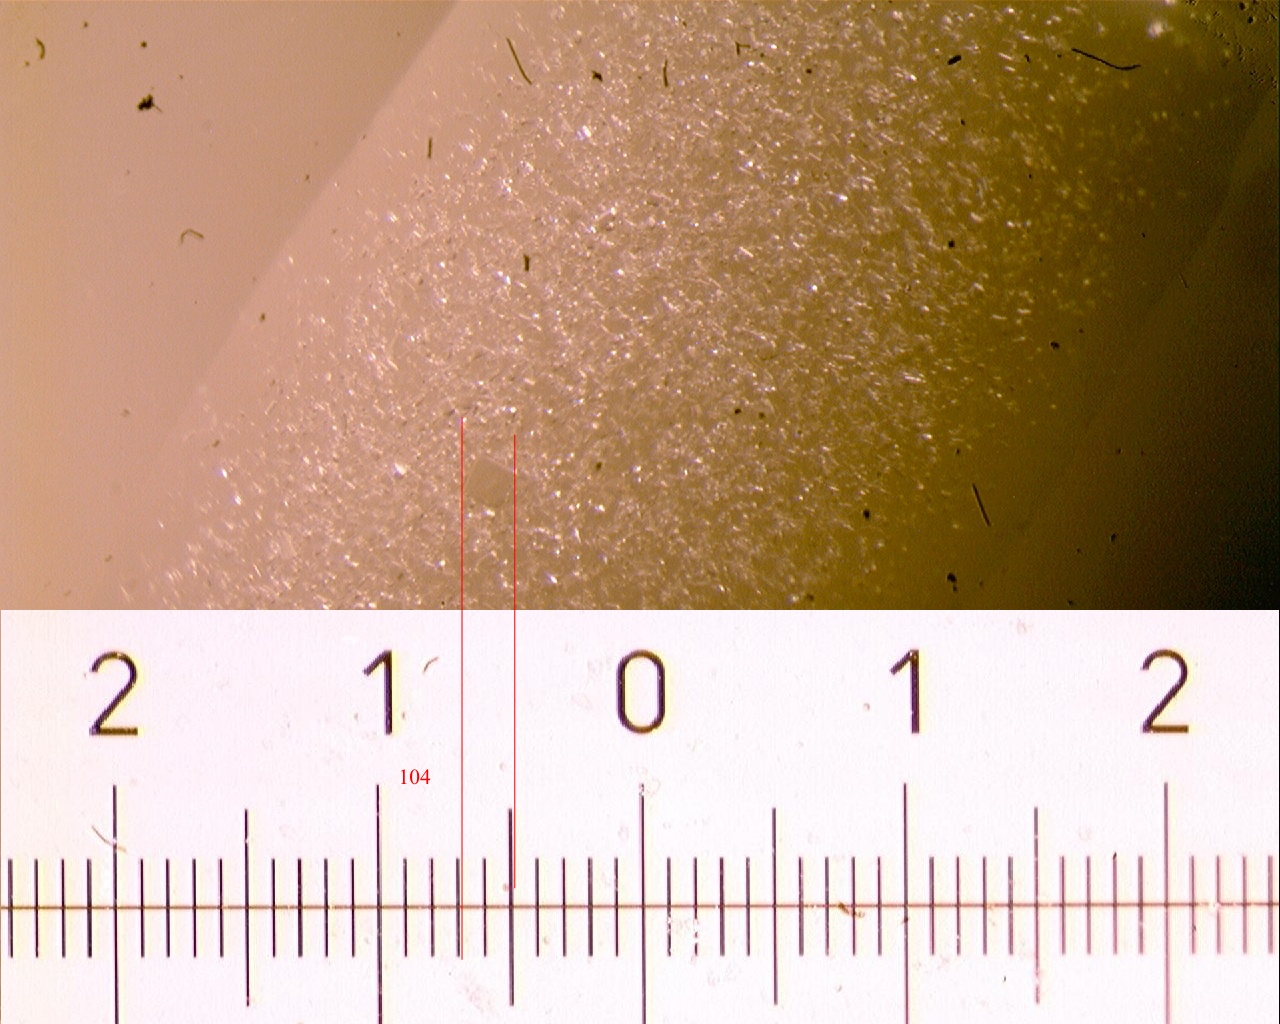
\includegraphics[width=0.9\textwidth]{2. First draft of protein crystalization/Images/labelled-Image-8_2000-01-21.jpg}
	    \caption{The largest crystal. The ruler image has 1278 × 453 pixels, and the droplet image has 1280 x 1024 pixels. The length of the largest crystal is 104 micrometers(52 pixels).  }
\end{figure}

-pH = 4.4: In terms of the number of crystals in the images, many small crystals were observed under the concentration of NaCl from 5\% to 8\%, while some small crystals could be observed under the NaCl concentration of 4\% and 9\%. As for crystal size, large crystals appeared at 4\%, 6\% and 9\% NaCl. The presence of crystals indicates that these protein solutions entered the supersaturated region. The emerging of large crystals at 4\% ,6\%, 9\% NaCl suggests that these protein solutions reached the metastable region after some crystals precipitated.


%All protein solutions start in the supersaturated region. However, the solubility of the protein is higher under 4\% NaCl, 6\% NaCl and 9\% NaCl, indicating that the protein solution will transition into the metastable region after nucleation.\\

-pH = 4.8: In terms of the number of crystals in the images, many small crystals were observed under the concentration of NaCl from 4\% to 9\%. As for crystal size, large crystals appeared at 4\% and 7\% to 9\% NaCl. The presence of crystals indicates that these protein solutions entered the supersaturated region. The emerging of large crystals at 4\% and 7\% to 9\% NaCl suggests that these protein solutions reached the metastable region after some crystals precipitated.\\


-pH = 5.2: In terms of the number of crystals in the images, many small crystals were observed under the concentration of NaCl from 6\% to 8\%, While few crystals could be observed at 4\%, 5\% and 9\% NaCl. As for crystal size, large crystals appeared at 4\% NaCl. The presence of crystals indicates that these protein solutions entered the supersaturated region. However, the few crystal in some groups indicates that they exited the supersaturated region soon. The emerging of large crystals at 4\% NaCl suggests that these protein solutions reached the metastable region after some crystals precipitated.\\

Finally, the largest crystal was found at the pH = 4.4, 6\% NaCl, with the length equals to 104$\pm $2$\mu$m.(Figure 3.2)\\

According to the findings in the previous study \hyperref[sec:ref_5]{[5]}, the solubility of the protein shows a positive correlation with the concentration of NaCl and pH within the range of our experiments. When analyzing our experiment in light of the previous study, it is expected that if large crystals appear in one group, they would also appear in the group with a higher pH and higher NaCl concentration,  which is not replicated by our results in this experiments. This may be attributed to experimental operations. It is hard to transfer 1 $\mu$l solution using the pipettes in the lab, which may influence the ratio of protein solution and buffer. Improving the pipetting could solve these issues mentioned.

\chapter{Reference}
[1]\label{sec:ref_1} : McPherson A, Gavira JA. Introduction to protein crystallization. Acta Crystallogr F Struct Biol Commun. 2014 Jan;70(Pt 1):2-20. doi: 10.1107/S2053230X13033141. Epub 2013 Dec 24. PMID: 24419610; PMCID: PMC3943105. \\

[2]\label{sec:ref_2} : McPherson, A. (1999). Crystallization of Biological Macromolecules. New York: Cold Spring Harbor Laboratory Press.\\

[3]\label{sec:ref_3} : Du M, Hou Z, Liu L, Xuan Y, Chen X, Fan L, Li Z, Xu B. 1Progress, applications, challenges and prospects of protein purification technology. Front Bioeng Biotechnol. 2022 Dec 6;10:1028691. doi: 10.3389/fbioe.2022.1028691. PMID: 36561042; PMCID: PMC9763899.\\

[4]\label{sec:ref_4} : Protein Crystallization, Biophysics lab course, Ulm University.\\

[5]\label{sec:ref_5} : Inyang, U.E., Iduh, A.O. Influence of pH and salt concentration on protein solubility, emulsifying and foaming properties of sesame protein concentrate. J Am Oil Chem Soc 73, 1663–1667 (1996). https://doi.org/10.1007/BF02517969\\

%[5]\label{sec:ref_5} : 
\end{document}
